\documentclass[11pt]{article}
\usepackage[utf8]{inputenc}
\usepackage{geometry}
\usepackage{graphicx}
\usepackage{hyperref}
\usepackage{amsmath}
\usepackage{listings}
\usepackage{xcolor}
\usepackage{float}

% Set page margins
\geometry{a4paper, margin=1in}

% Set up code listing style
\lstset{
    basicstyle=\ttfamily,
    commentstyle=\color{gray},
    keywordstyle=\color{blue},
    stringstyle=\color{red},
    showstringspaces=false,
    captionpos=b
}

\title{Development of a Sudoku Solver: C1 Research Computing Coursework}
\author{Vishal Jain}
\date{\today}

\begin{document}

\maketitle

\tableofcontents

\newpage

\section{Introduction}

\begin{quote}
    "Sudoku is a denial of service attack on human
  intellect" - Ben Laurie
\end{quote}

This report details the development of a Sudoku solver inline with the requirements of the C1 Research Computing coursework. The programme takes as input an incomplete grid in the form of a text file with a 9x9 grid of numbers with zero representing unknown values and `|`,`+`,`-` separating cells and , i.e.:


\begin{verbatim}
    $ cat input.txt
    000|007|000
    000|009|504
    000|050|169
    ---+---+---
    080|000|305
    075|000|290
    406|000|080
    ---+---+---
    762|080|000
    103|900|000
    000|600|000
    \end{verbatim}

and outputs the completed grid in the same form.


\section{Problem Decomposition}
To architect the Sudoku solver program, an initial flowchart was constructed to map out the high-level logical sequence. Each step of the flowchart was assigned a color based on its logical independence. This method helped identify distinct, modular components within the program's workflow. The resulting color-coded flowchart is presented in Figure \ref{fig:solver_flowchart}.


The analysis led to the identification of the following key modular components in the Sudoku solver:

\begin{itemize}
\item \textbf{User IO:} Responsible for user interaction and input/output processing.
\item \textbf{Format Validation:} Ensures the correctness of the input format.
\item \textbf{Board Logic:} Manages the internal representation and manipulation of the Sudoku board.
\item \textbf{Solver Logic:} Implements the algorithms to solve the Sudoku puzzle.
\end{itemize}


\subsection{Developmental Journey}
Before delving into the final structure of the Sudoku solver, it is insightful to explore the initial prototyping phase. This phase laid the groundwork for the project and provided key insights that shaped the final design.

\begin{figure}[H]
\centering
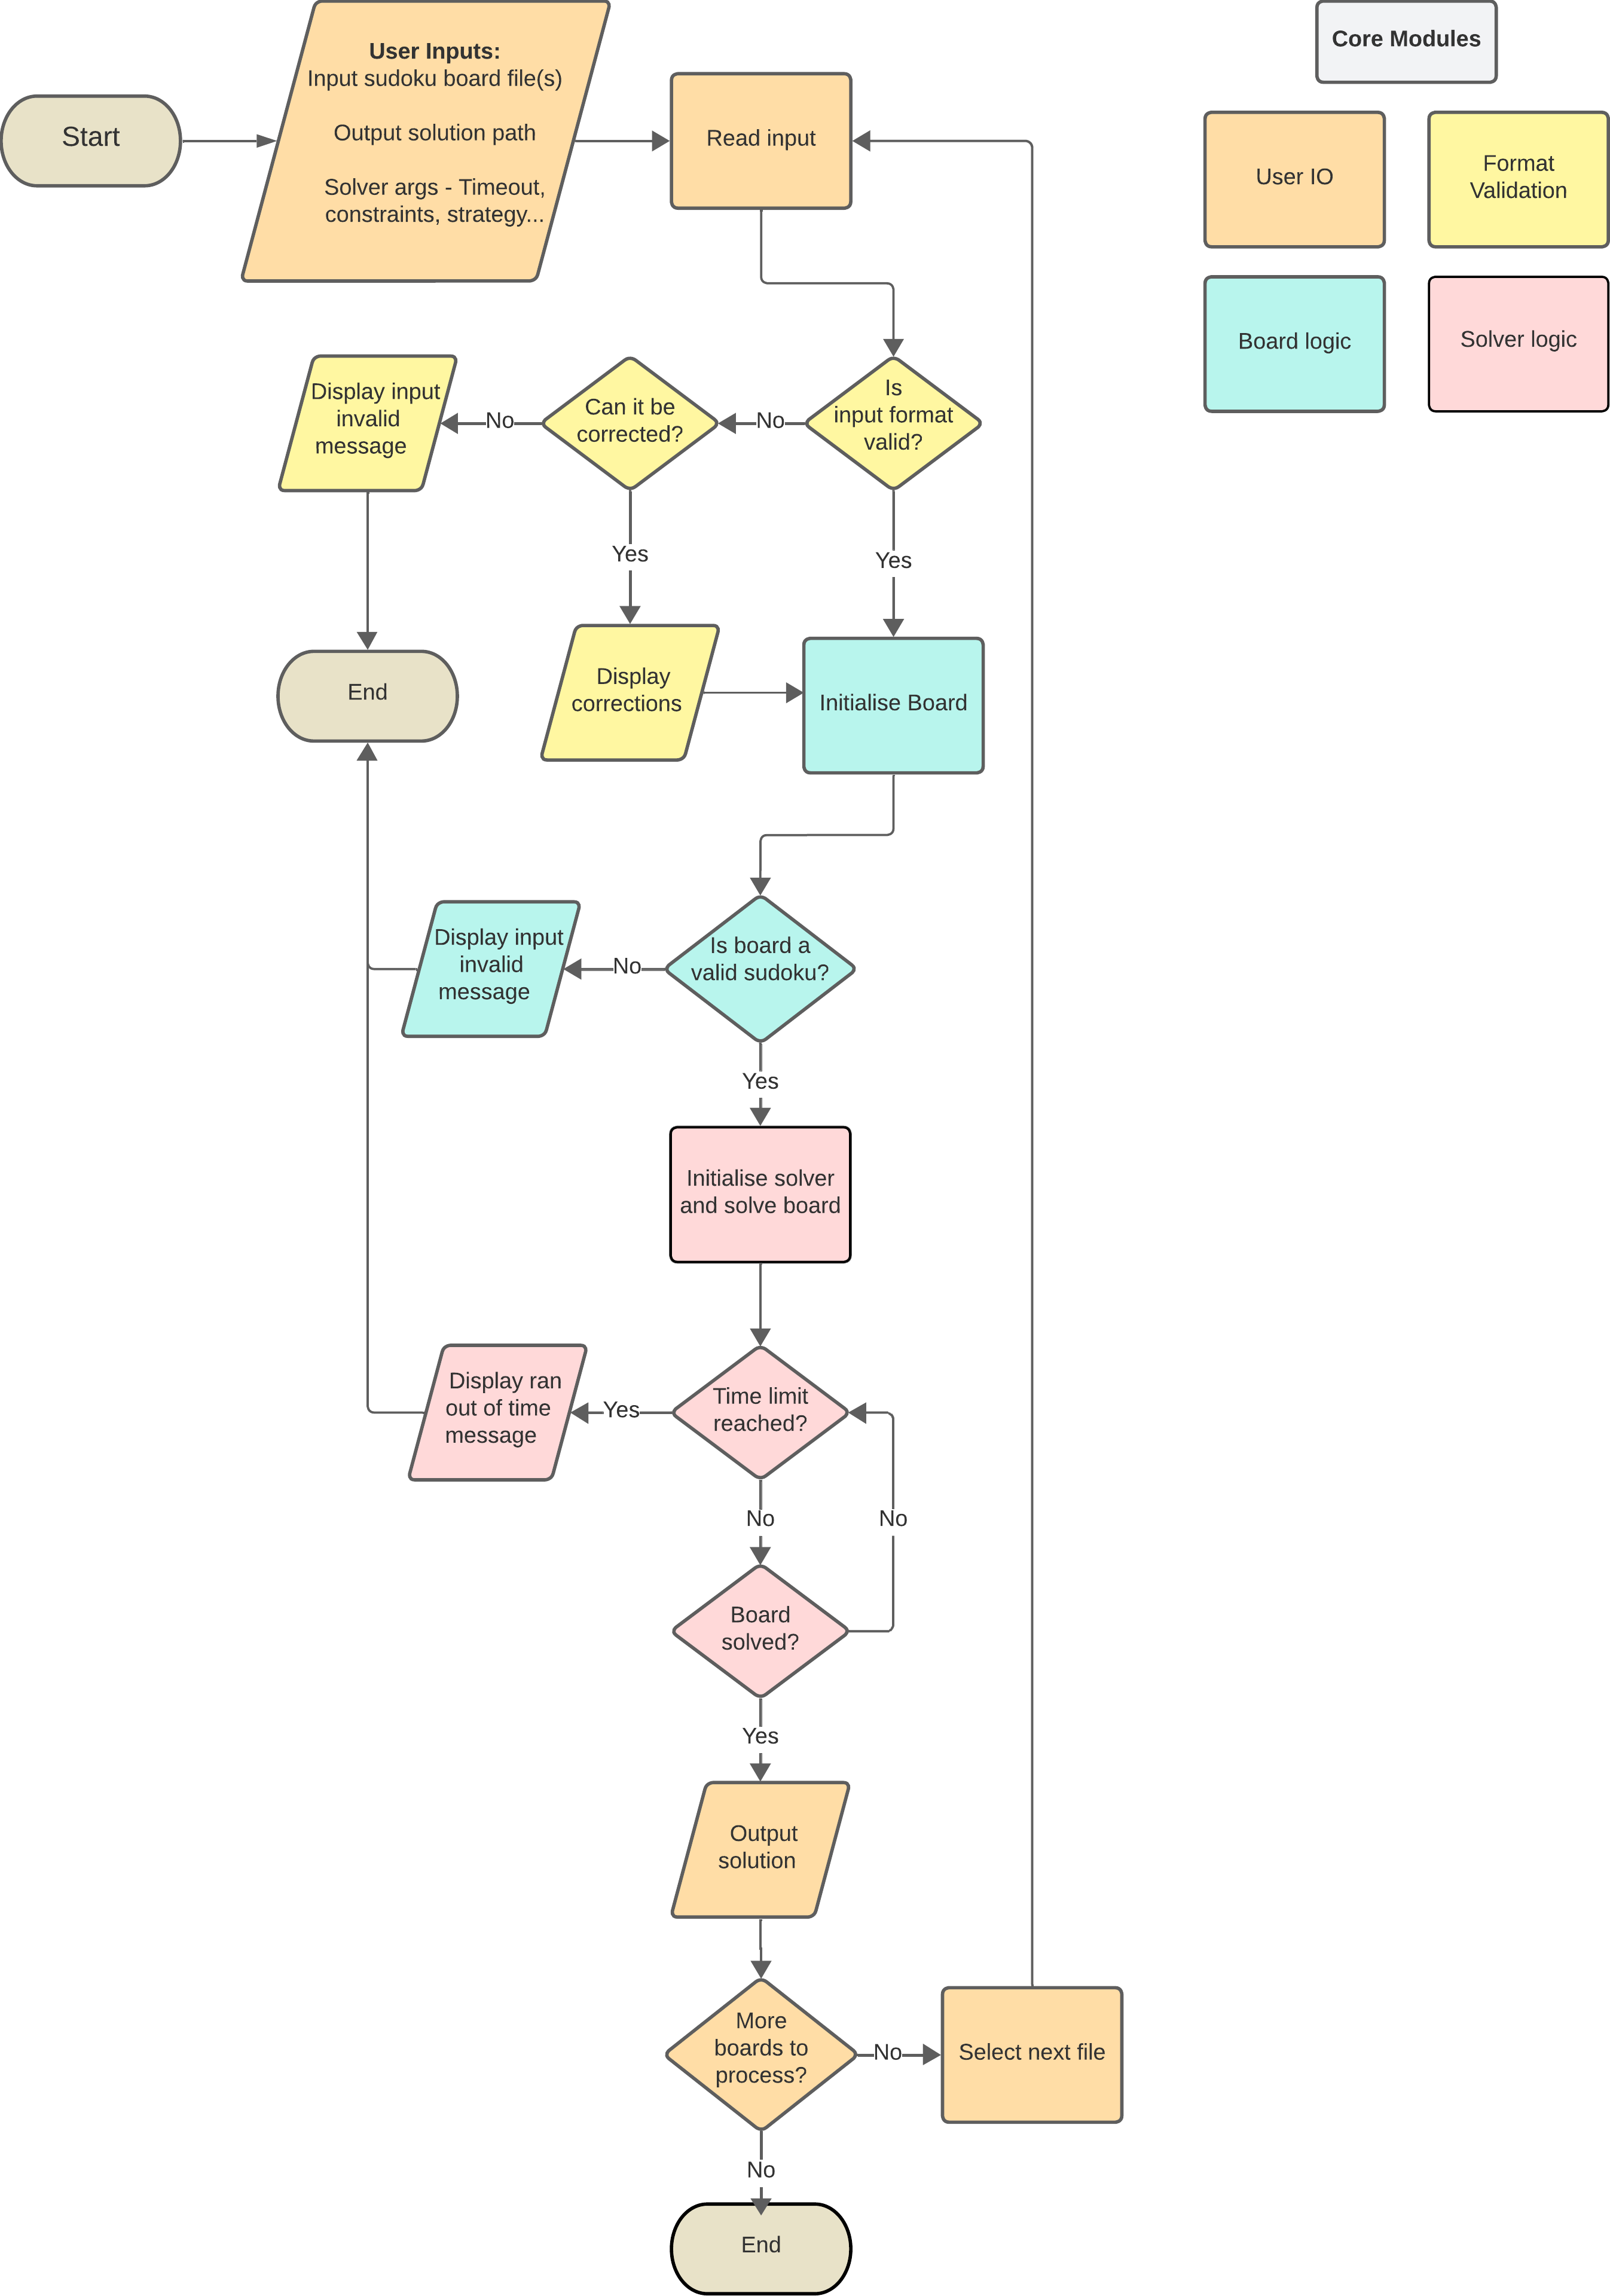
\includegraphics[width=1\textwidth]{figs/solver_flowchart.png}
\caption{High-level flowchart of the Sudoku solver program, illustrating the initial conceptual design. Functionally related modules are color-coded: orange for user interaction, yellow for format validation, cyan for board logic, and pink for solver logic components.}


\label{fig:solver_flowchart}
\end{figure}

\subsubsection{Early Prototyping}
In the initial stages, the envisioned usage of the program was conceptualised as a straightforward sequence of operations involving board validation, board representation, and solving. The logical flow was as follows:

\begin{enumerate}
\item \textbf{Board Validation}: The user provides a file containing the Sudoku puzzle, which is then read, validated, and corrected if necessary. This process was handled by a utility function, \texttt{validate\_board}, located in the \texttt{utils} module. The function's purpose was to ensure the input adhered to Sudoku format standards and to correct any discrepancies. The code snippet for this step:
\begin{verbatim}
board_array = utils.validate_board(board_file)
\end{verbatim}
This function returns a 9x9 array representing the initial state of the Sudoku board.

\item \textbf{Board Representation}: The returned board array is then used to initialise an instance of the `\texttt{SudokuBoard}` class. This class encapsulates the board's representation and manipulation logic, providing common game board methods like `\texttt{reset}` and `\texttt{check\_valid}`. The initialisation step is shown below:
\begin{verbatim}
board = SudokuBoard(board_array)
\end{verbatim}

\item \textbf{Solving the Puzzle}: Finally, the `\texttt{SudokuBoard}` instance is passed to the `\texttt{solve}` method of a `\texttt{BacktrackingSolver}` class instance. The solver applies the backtracking algorithm to find a solution to the puzzle, returning a new `\texttt{SudokuBoard}` instance representing the solved board:
\begin{verbatim}
solved_board = BacktrackingSolver(board).solve()
\end{verbatim}

\end{enumerate}


\subsubsection{Early Hurdles and Insights in Sudoku Solver Development}
Trying to test the prototyped solution on a kaggle datasets of a million sudoku puzzles, lead to the following issues and insights.
\begin{itemize}
\item \textbf{Multiple Input Formats:} Handling non-grid formats, like Kaggle's single line format, was problematic, underscoring the need for native support for various formats and more efficient format conversion.
\item \textbf{Modularity Challenges:} Initially, \texttt{validate\_board} was a singular function for board validation, correction, and parsing, which limited flexibility and complicated handling diverse input formats.
\item \textbf{SudokuBoard's Role:} The \texttt{SudokuBoard} class struggled with dual roles as both user interface and board representation. Its \texttt{save} method became problematic with multiple format support. Additionally, its responsibility to validate Sudoku boards was improperly outsourced to an external utility, leading to unclear responsibilities and disjointed design.

\item \textbf{Solver Extensibility:} The initial design poorly accommodated diverse solver algorithms, particularly those requiring unique initialisation, highlighting the need for a more adaptable system for new solver integration.

\item \textbf{Input Flexibility:} \texttt{main.py} was initially not equipped to handle directories of board files, dynamic solver or format selection, and string inputs, the latter emerging as a key feature for rapid puzzle testing.
\end{itemize}


\subsubsection{High-Level Overview of the Final Implementation}
The final design of the Sudoku solver program encapsulates a modular and flexible architecture, as outlined below:

\begin{verbatim}
# Initialise the Format Handler and Solver
format_handler = SudokuFormatHandler()
solver = SudokuSolver()

# Parse the Sudoku board from the given input in the desired format
board = format_handler.parse(board_file, format_type)

# Employ a specific solver to find a solution for the parsed board 
solved_board = solver.solve(board, solver_backend)

# Save the solved board in the desired format and output path
format_handler.save(solved_board, format_type, output_path)
\end{verbatim}

In this design, \texttt{SudokuFormatHandler} and \texttt{SudokuSolver} act as wrapper classes that have methods which allow the user to specify which format and solver backend they want to use, respectively. These classes utilise standardised methods to process and solve the Sudoku puzzle, irrespective of the specific format or solving algorithm used. This approach significantly enhances the extensibility of the program, allowing for the easy integration of new formats and solving methods without requiring changes to the \texttt{main.py} script. The next section will explore the design and implementation of the various modules in greater detail.

\section{Programme Modules}
\subsection{SudokuFormatHandler Class}

\subsubsection{Scope}
The scope of the \texttt{FormatHandler} classes implemented in \texttt{src/sudoku\_format\_handler.py} are defined by their role in bridging the gap between external representations of Sudoku boards and standardised internal representation. Specifically, the scope of this class encompasses:

\begin{itemize}
\item \textbf{Parsing}: Handling the conversion of the input, whether it comes as a string or as a file path, into a standardised \texttt{SudokuBoard} object.

\item \textbf{Saving}: Conversely, the class also manages the conversion of \texttt{SudokuBoard} objects back into user-readable formats. 

\item \textbf{Format Validation and Correction}: This class is also where the developer defines any methods for validation checks and corrections to ensure that the input is in the expected format before parsing.
\end{itemize}

\subsubsection{Design and Implementation}
The design of the \texttt{SudokuFormatHandler} class is centered around principles of modularity and extensibility, driven by the use of an abstract base class and a handler dictionary. Key design aspects include:

\begin{itemize}
    \item \textbf{Modularity}: The class leverages an abstract base class, \texttt{FormatHandler}, which outlines essential methods -- \texttt{parse} and \texttt{save}. This structure ensures consistency across different format handlers while allowing for flexibility in their specific implementations.
    \item \textbf{Extensibility}: New formats can be easily integrated into the system by creating a subclass of \texttt{FormatHandler} and adding it to \texttt{SudokuFormatHandler}'s \texttt{handler\_dict} class attribute. This approach simplifies the process of extending the system to accommodate new Sudoku board formats.
\end{itemize}
The UML class diagrams in Figure \ref{fig:format_handler_uml} provide a visual representation of the design and implementation of the \texttt{FormatHandler} abstract base class and the concrete grid and line format handler classes used by the \texttt{SudokuFormatHandler} class.
\begin{figure}[H]
    \centering
    \includegraphics[width=1\textwidth]{figs/UML_sudoku_handler.png}
    \caption{UML class diagram for implementation of the FormatHandler classes. Abstract classes are depicted in pink, concrete classes in blue. Composition relationships are indicated with arrows having a white diamond base and a solid head.}
    \label{fig:format_handler_uml}
\end{figure}


\paragraph{GridFormatHandler}
The GridFormatHandler is the format handler for the required format of this coursework. It is designed to handle the parsing and saving of Sudoku boards in the grid format. The parsing process involves reading the input file or string and converting it into a list of strings representing each row of the Sudoku board. The white space and empty lines are removed. Any dots are replacecd with zeros as this is commonly seen online as a placeholder for empty cells. The handler ensures there are exactly 11 rows; otherwise, it raises an error. Each row undergoes validation against a specific regex pattern. If a row deviates from the expected pattern but aligns with an alternate acceptable one, it undergoes correction; otherwise, an error is raised. Correction logic is applied selectively: Separator rows lacking numbers are replaced with a standard separator row, but if they contain numbers, an error is raised to avoid digit alteration. For a row which is expected to describe a number row, if it matches the general pattern of 3 sets of numeric character triplets seperated by a non numeric character, it is corrected by inserting the expected seperator characters between the triplets.

\subsubsection{Extensibility}
The\texttt{SudokuFormatHandler} is designed with extensibility in mind. To support a new format, a developer simply needs to create a new handler class extending \texttt{FormatHandler} and implement the \texttt{parse} and \texttt{save} methods with the expected inputs and outputs. The new handler can then be added to the \texttt{handler\_dict}. This design makes it straightforward to extend the solver's capabilities to accommodate future requirements or user preferences for different Sudoku board formats.


\subsubsection{Limitations}
The SudokuFormatHandler module and related components are designed for processing single Sudoku boards from individual files. This approach reduces complexity compared to a general framework handling multiple formats and boards in one file. By adhering to a single input, single board model, the program remains simpler and more predictable, minimising unexpected behaviors.

\subsection{SudokuBoard Class}

\subsubsection{Scope}
The \texttt{SudokuBoard} class in \texttt{src/sudoku\_board.py} is integral to managing the internal representation and manipulation of the Sudoku board and providing a standardised interface for the other classes in the program. The scope of this class encompasses:

\begin{itemize}
    \item \textbf{Board Validation}: Makes sure board state always follows Sudoku rules. 
    \item \textbf{Board Representation}: Provides a standardised representation of the board state for the other classes. 
    \item \textbf{Board Manipulation}: Facilitates methods for resetting the board and modifying cell values to allow for board manipulation.
    \item \textbf{Solving Assistance}: Provides common utility methods required by typical solvers, such as fetching empty cells and checking valid number placements.

\end{itemize}
\subsubsection{Design and Implementation}

The design of the \texttt{SudokuBoard} class adheres to the principle of encapsulation, ensuring that the internal state of the board is managed in a controlled manner. This class serves as the central interface for other components of the program, providing standardised methods to interact with the Sudoku board.

\begin{itemize}
\item \textbf{Array-like Access}: The class maintains encapsulation by hiding the underlying board structure. It provides an array-like interface for read-only access to board elements using the \texttt{\_\_getitem\_\_} method. This approach enables intuitive indexing while protecting the board's state from external modifications.

\item \textbf{Board Representation and Validation}: Internally, the class uses a 2D numpy array for the board's representation, accompanied by sets for efficient tracking of existing numbers in rows, columns, and 3x3 subgrids, facilitating quick validation checks.

\item \textbf{Controlled Board Manipulation}: To preserve the integrity of the board's state, direct modification methods like setters are omitted. Instead, specific methods like \texttt{place\_number} and \texttt{remove\_number} are provided. These methods ensure that all changes to the board follow Sudoku rules and constraints.

\item \textbf{Convenience Methods}: The class offers various utility methods such as resetting the board and finding empty cells. These methods simplify common operations required for solving Sudoku puzzles.

\item \textbf{Initialisation and Formatting}: The \texttt{\_\_init\_\_} method checks initial state represents a valid sudoku board. The \texttt{\_\_str\_\_} method provides a human-readable string representation of the board, enhancing the ease of debugging and visualisation.
\end{itemize}

The UML class diagram in Figure \ref{fig:sudoku_board_uml} provides a visual representation of the implementation of the \texttt{SudokuBoard} class.

\begin{figure}[H]
    \centering
    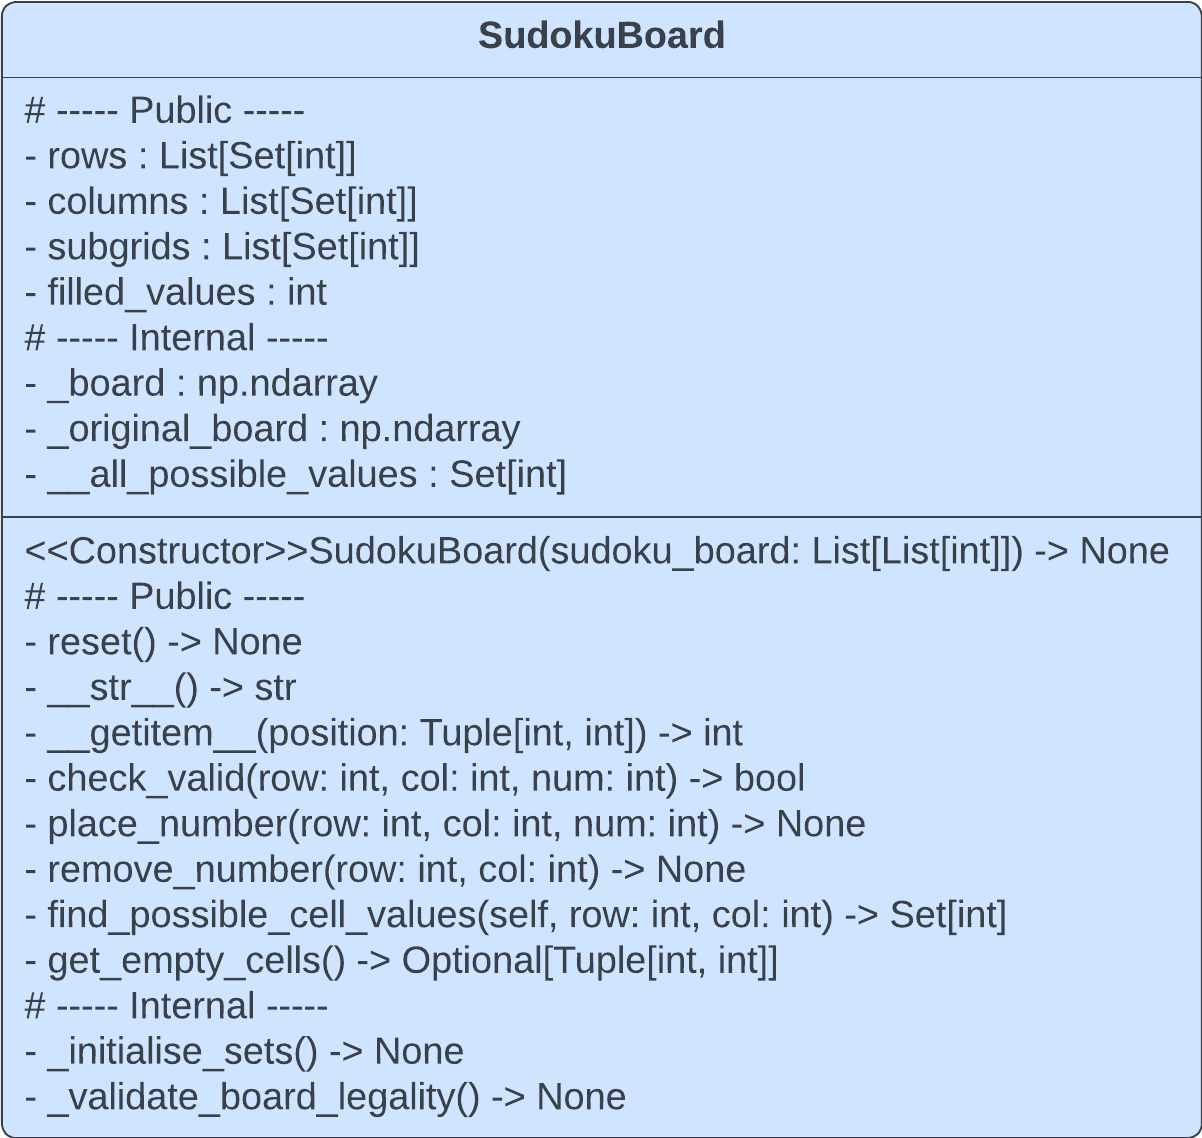
\includegraphics[width=0.5\textwidth]{figs/UML_sudoku_board.png}
    \caption{UML class diagram for the SudokuBoard module.}
    \label{fig:sudoku_board_uml}
\end{figure}
 
\subsubsection{Extensibility and Limitations}
The \texttt{SudokuBoard} class, unlike \texttt{SudokuFormatHandler}, isn't inherently extensible for different board types such as dictionary representations. To address this, an abstract \texttt{Board} base class could be introduced, defining the common methods for solvers and format handlers with their expected inputs and outputs. \texttt{SudokuBoard} would then act as a wrapper class, instantiating the specific concrete \texttt{Board} implementations specified by the user.


\subsection{SudokuSolver Class}
\subsubsection{Scope}
The scope of the \texttt{SudokuSolver} class in \texttt{src/sudoku\_solver.py} is defined by the following:
\begin{itemize}
    \item \textbf{Solving}: Taking in a \texttt{SudokuBoard} object and returning a solved \texttt{SudokuBoard} object.
    \item \textbf{Outputting Solve Status}: Returning the status of the solution, eg whether the board has no solution, ran into timeout, or was solved successfully.
    \item \textbf{Algorithm Selection}: Providing a standardised interface for selecting the implemented solving algorithm.
\end{itemize}
\subsubsection{Design and implementation}
\begin{itemize}
    \item \textbf{Modularity}: The class leverages an abstract base class, \texttt{Solver}, which outlines the essential method for all solvers -- \texttt{solve}. This structure ensures consistency across different solvers while allowing for flexibility in their specific implementations.
    \item \textbf{Extensibility}: New solvers can be easily integrated into the system by creating a subclass of \texttt{Solver}. After implementation, to use it just add it to \texttt{SudokuSolvers}'s \texttt{solver\_dict} class attribute and call the \texttt{set\_solver} method with the desired solver backend to select it.
\end{itemize}

The UML class diagrams in Figure \ref{fig:sudoku_solver_uml} provide a visual representation of the design and implementation of the \texttt{Solver} abstract base class and the \texttt{SudokuSolver} class along with the implemented \texttt{BacktrackingSolverBasic} and {BacktrackingSolverEasiestFirst} classes.

\begin{figure}[H]
    \centering
    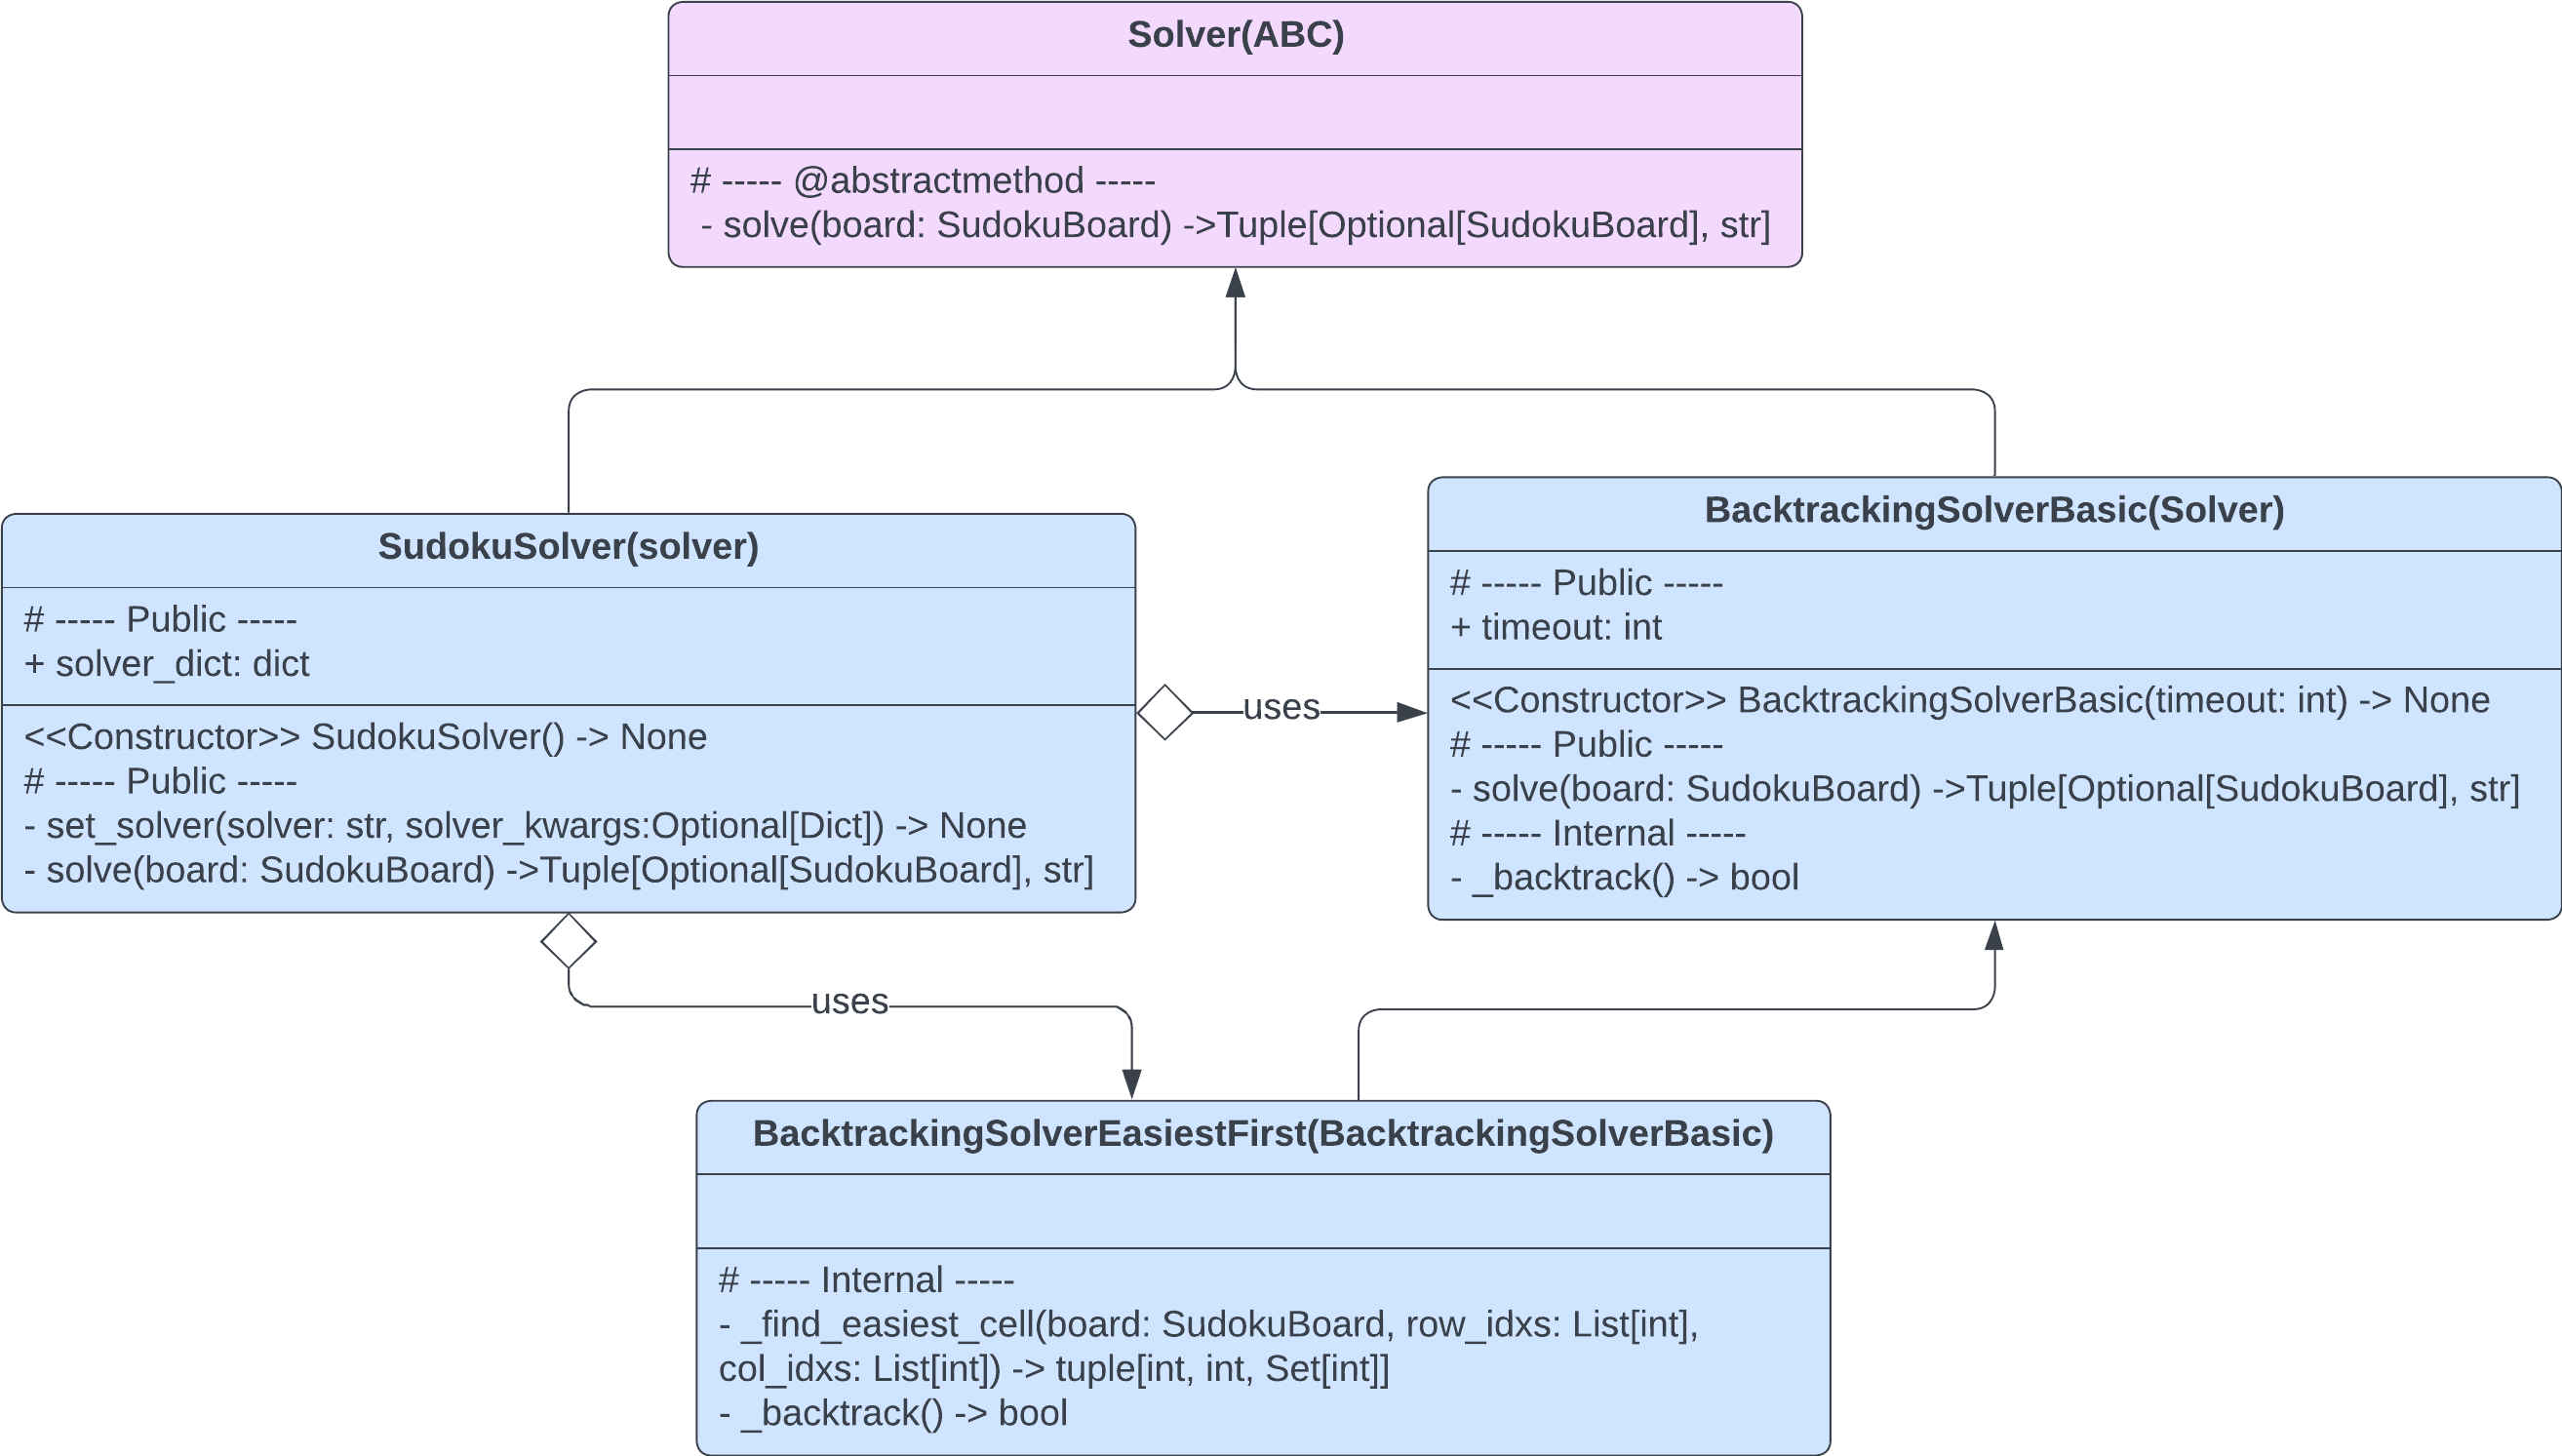
\includegraphics[width=1\textwidth]{figs/UML_sudoku_solver.png}
    \caption{UML class diagram for implementation of the SudokuSolver classes. Abstract classes are depicted in pink, concrete classes in blue. Composition relationships are indicated with arrows having a white diamond base and a solid head.}
    \label{fig:sudoku_solver_uml}
\end{figure}

\paragraph{Backtracking-Based Sudoku Solvers:}

The types of solver implemented in this coursework are based on the method of backtracking. Backtracking is a straightforward brute-force method that uses recursive depth-first search to explore all possible solutions, starting from the initial state of the Sudoku board. This method systematically tries every valid option for each empty cell and backtracks when it reaches a state where it can't make any valid moves.

While this approach is comprehensive, it's not particularly efficient because it doesn't use heuristics—techniques to speed up the process by eliminating unlikely paths. Consequently, it can be very slow on certain boards which require very deep exploration to find a solution. 

Here, two backtracking based solvers are implemented: \texttt{BacktrackingSolverBasic} and \texttt{BacktrackingSolverEasiestFirst}. The former is a basic implementation of the backtracking algorithm, while the latter uses a heuristic to prioritise cells with the fewest possible values, reducing the number of possibilities to explore. The \texttt{BacktrackingSolverEasiestFirst} solver is the default solver used by the \texttt{SudokuSolver} class.

The performance of the solvers was evaluated using two distinct datasets: a set of 1 million Sudoku puzzles sourced from Kaggle \cite{kaggleDataset}, and a collection of 100 puzzles known to challenge backtracking algorithms which can be found in the repository at the path \texttt{benchmark\_board\_sets/hard\_100}. A timeout limit of 30seconds is set to avoid the solver getting stuck on a puzzle. The results are shown in Table 

The backtracking with the easiest first heuristic is slightly slower than the basic backtracking solver on the easy puzzles, but significantly faster on the hard puzzles. 
\begin{figure}[h!]
    \centering
    \begin{tabular}{|c|c|c|}
    \hline
    Solve Time Metric & Basic & Easiest First \\
    \hline
    Median (ms) & 0.569 & 1.32 \\
    \hline
    Average (ms) & 0.773 & 1.35 \\
    \hline
    Max (ms) & 96.6 & 132 \\
    \hline
    Min (ms) & 1.47 & 1.12 \\
    \hline
    Std (ms) & 0.782 & 0.492 \\
    \hline
    \end{tabular}
    \caption{Comparison of basic backtracking vs backtracking with easiest first heuristic performance metrics on the Kaggle million dataset.}
\end{figure}

\begin{figure}[h!]
    \centering
    \begin{tabular}{|c|c|c|}
    \hline
    Solve Time Metric & Basic & Easiest First \\
    \hline
    Median (s) & 1.100 & 0.083 \\
    \hline
    Average (s) & 9.726 & 0.706 \\
    \hline
    Max (s) & 120.000 & 12.028 \\
    \hline
    Min (ms) & 1.470 & 2.230 \\
    \hline
    Std (s) & 22.115 & 1.968 \\
    \hline
    \end{tabular}
    \caption{Performance metrics comparison: basic backtracking vs easiest first heuristic on 100 puzzles optimised for backtracking challenge.}


\end{figure}

\subsubsection{Extensibility and Limitations}
The Sudoku solver system is designed for easy extensibility. Developers can add new solvers by creating a class that extends \texttt{Solver} and implements the \texttt{solve} method with appropriate inputs and outputs. For backtracking solvers, extending \texttt{BacktrackingSolverBasic} and implementing \texttt{\_backtrack} suffices. New solvers are integrated into the system by adding them to the \texttt{solver\_dict} in the \texttt{SudokuSolver} class.

However, the system currently operates on a single-threaded execution model, not utilizing parallel processing which could expedite solving by simultaneously exploring multiple solution tree branches. Additionally, while flexible within the backtracking approach, the framework might not easily support radically different solving methods.

\subsection{UserIO}
\subsubsection{Scope}
The user IO is handled by the \texttt{src/main.py} script. This script is defined by its role as the entry point for the Sudoku solver program. The scope of this script encompasses:

\begin{enumerate}
    \item \textbf{Argument Parsing and Validation:} Interprets and validates command-line arguments for configuring the solver's operation.
    \item \textbf{Initialisation:} Sets up core components like `\texttt{SudokuFormatHandler}` and `\texttt{SudokuSolver}` based on user inputs.
    \item \textbf{Solving Process Management:} Manages the Sudoku solving flow, accommodating both single and batch operations.
    \item \textbf{Statistics and Output Handling:} Gathers and presents solving statistics, handling outputs for solved puzzles.
\end{enumerate}

\subsubsection{Design and implementation}
The `main.py` script in the Sudoku solver program is underpinned by the following design principles:

\begin{itemize}
    \item \textbf{Backend Independence:} Maintains independence from the solver and format handler backends.
    \item \textbf{User Customisation:} Allows users to define input and output formats, enabling highly customised runs.
    \item \textbf{Reproducibility:} Facilitates reproducible runs by saving statistics, including the Git commit hash and run arguments.
    \item \textbf{Robust Error Handling:} Incorporates thorough argument validation and error handling to safeguard user interaction.
    \item \textbf{Intuitive Defaults with Customization Options:} Provides sensible defaults for ease of use, alongside a range of customisable arguments for advanced users.
    \item \textbf{Dynamic Solver and Formatter Integration:} Automatically enables selection of solvers and formatters added to the Sudoku solver and format handler.
    \item \textbf{Clear Output and Feedback:} Ensures outputs are easily understandable and provides clear user feedback throughout the process.
\end{itemize}

The implementation of logic is shown as a flow chart in Figure \ref{fig:main_flowchart}.

\subsubsection{Extensibility and Limitations}
The main way in which \texttt{main.py} is currently designed to be extensible is in the integration of more complex solvers. At present, solvers can be initialised with a singular timeout parameter. However, in anticipation of future more complex solvers which require more initialisation parameters, a space for that logic has been left in the get\_solver\_args function. This function, which currently takes as input the users arguments, can easily be designed to handle the parsing of an input configuration file. This capability paves the way for the incorporation of advanced solvers without necessitating substantial modifications to the existing codebase. 
The main limitation of main.py is that adding more output metrics like backtracking recursions, or other solver based statistics requires some plumbing work. Further, implementing parallel processing requires some code refactoring. 
\begin{figure}[H]
    \centering
    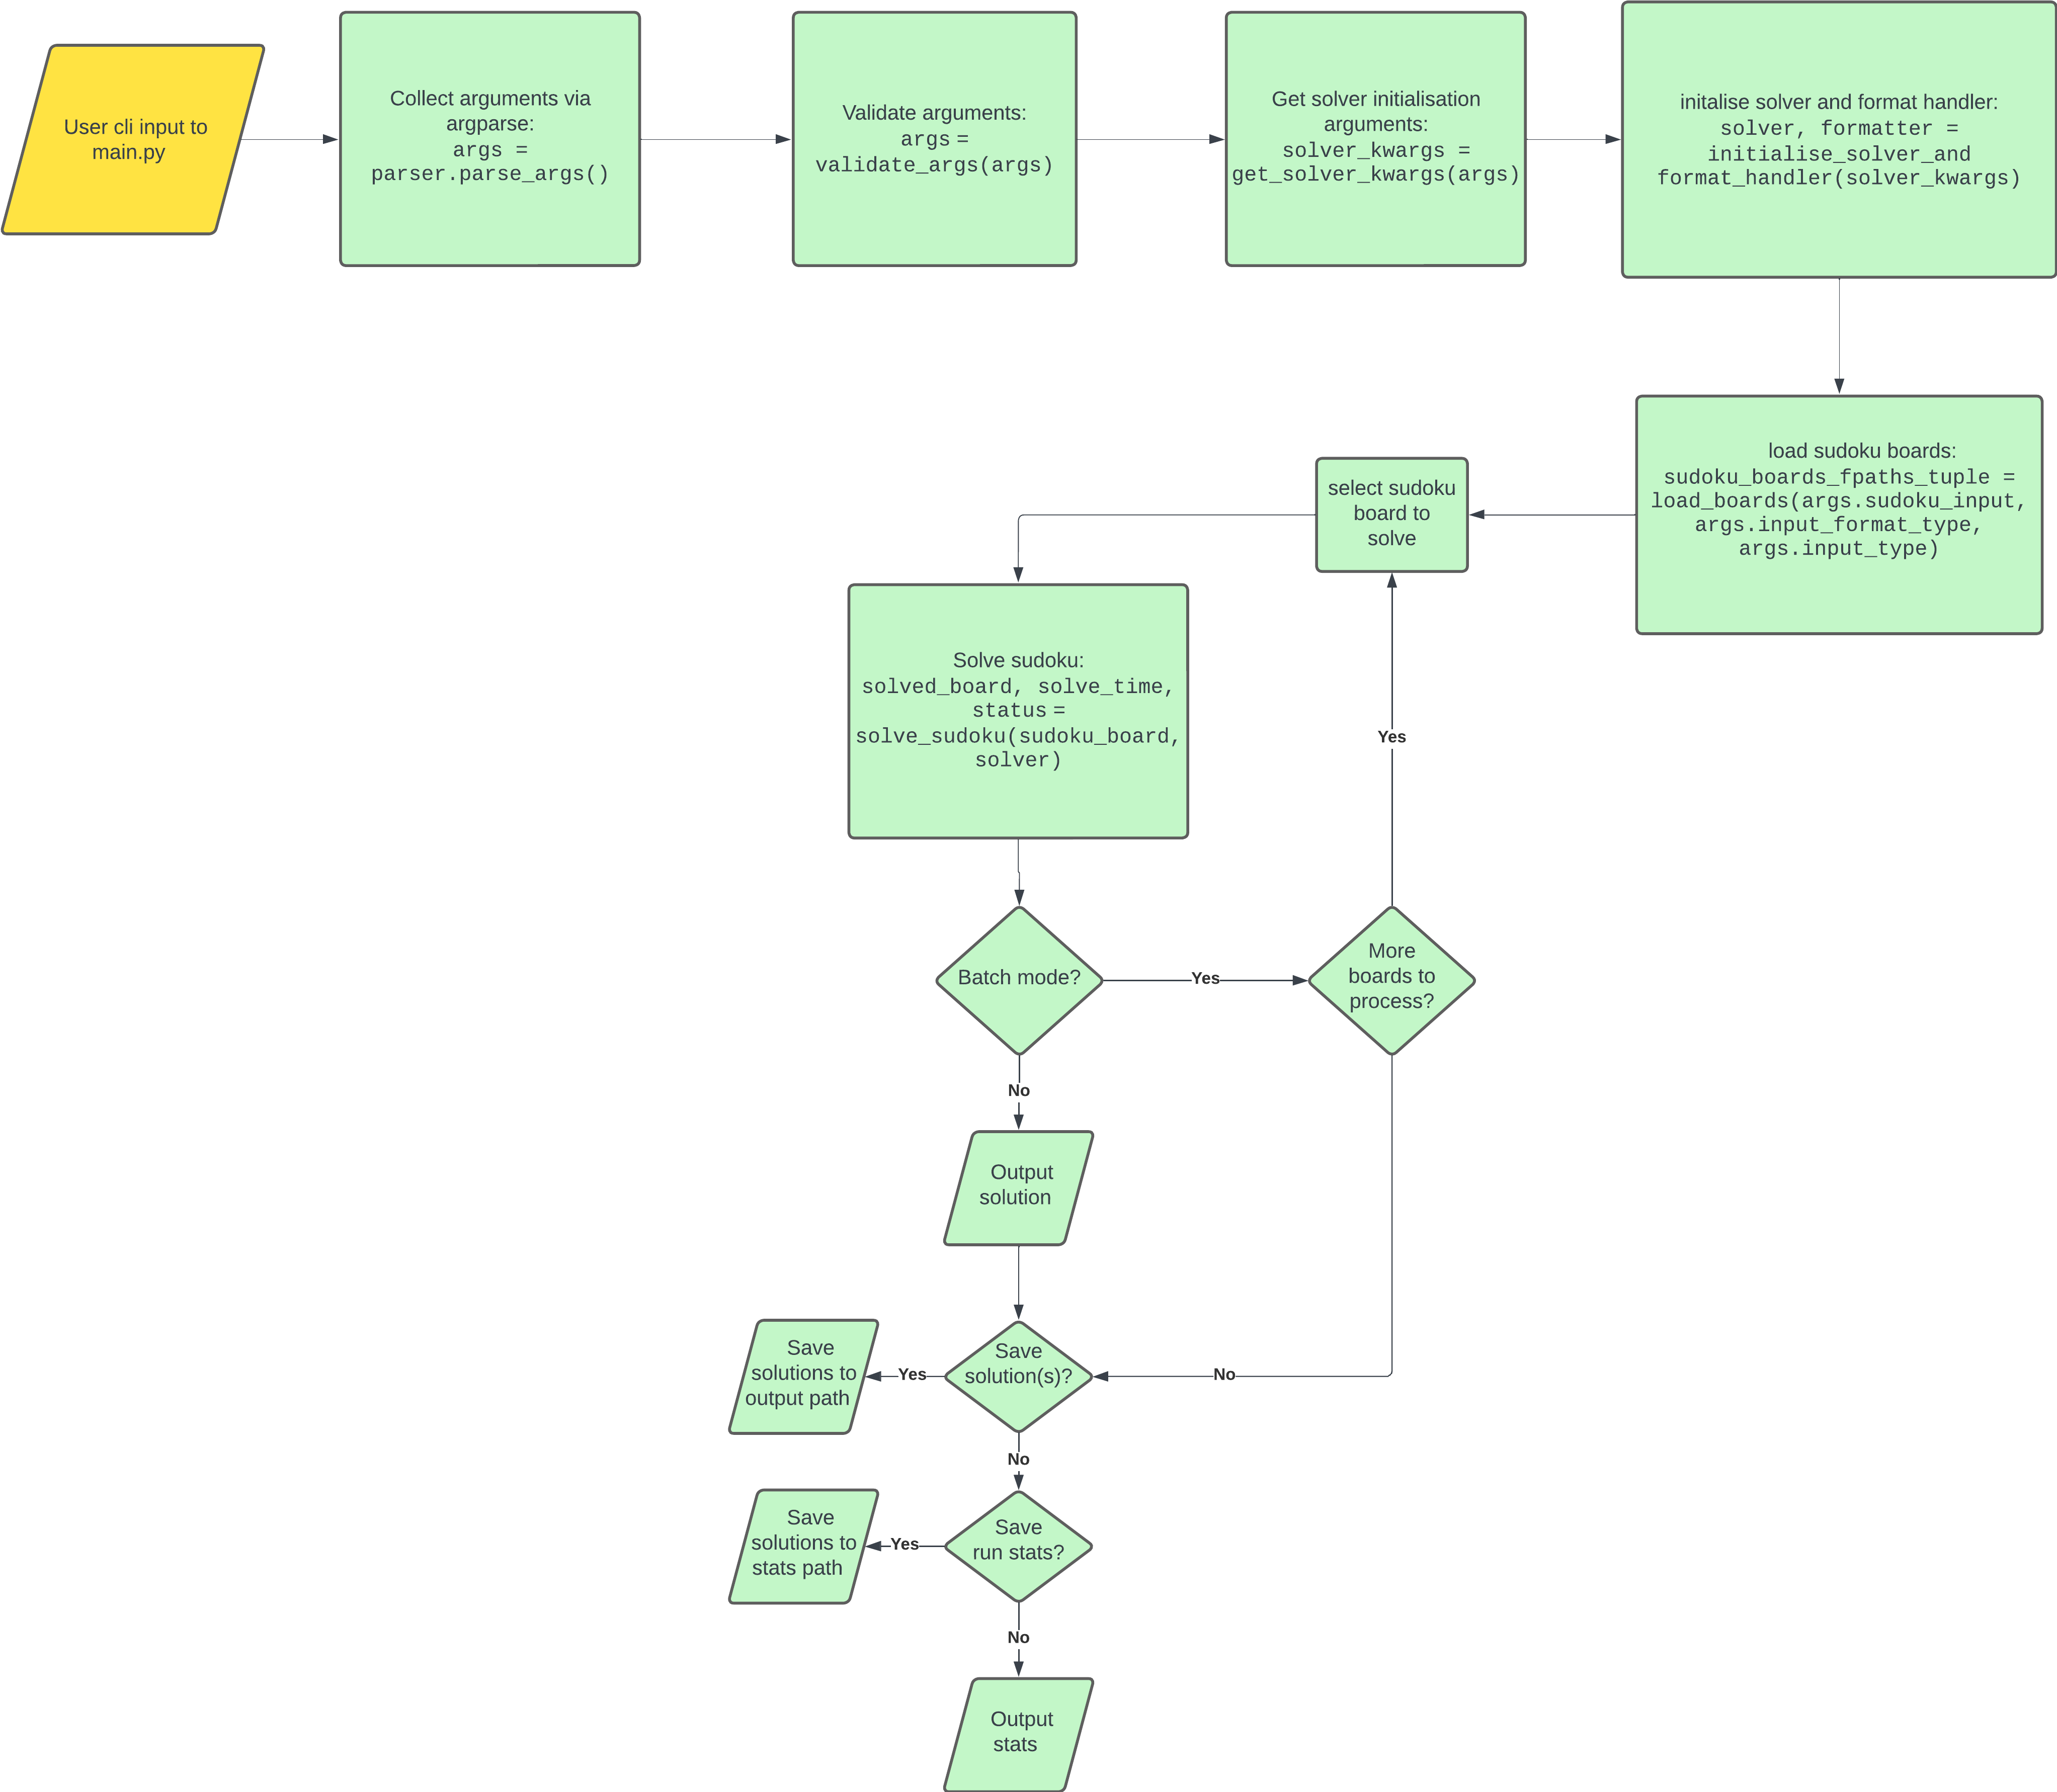
\includegraphics[width=1\textwidth]{figs/main_flowchart.png}
    \caption{Flowchart of the main.py script.}
    \label{fig:main_flowchart}
\end{figure}


\section{Profiling and optimisation}

To reproduce the line profiling results mentioned below, follow these steps:

\begin{verbatim}
# For the initial results 
git checkout 4c1278cf

# For the final results
# git checkout c3fad894

# Activate the environment (replace 'env_name' with your environment name)
source activate C1_VJ279

# Add @profile to the check_valid method of the SudokuBoard class
# Add @profile to the _backtrack method of the BacktrackingSolver class

# Run the line profiler on the difficult sudoku board
kernprof -l -v src/main.py test/challenging_boards/challenging_sudoku_0.txt
 --format_type flat
\end{verbatim}


The line profiling of the initial Sudoku solver highlighted two critical functions: the \texttt{check\_valid} method of \texttt{SudokuBoard} and the \texttt{\_backtrack} method of \texttt{BacktrackingSolver}. \texttt{check\_valid}, taking 242.043 seconds, was identified as a major performance bottleneck due to its frequent invocation by \texttt{\_backtrack}, which itself took 514.918 seconds with 91.5\% of this time spent on \texttt{check\_valid}. 
\begin{figure}[H]
    \centering
    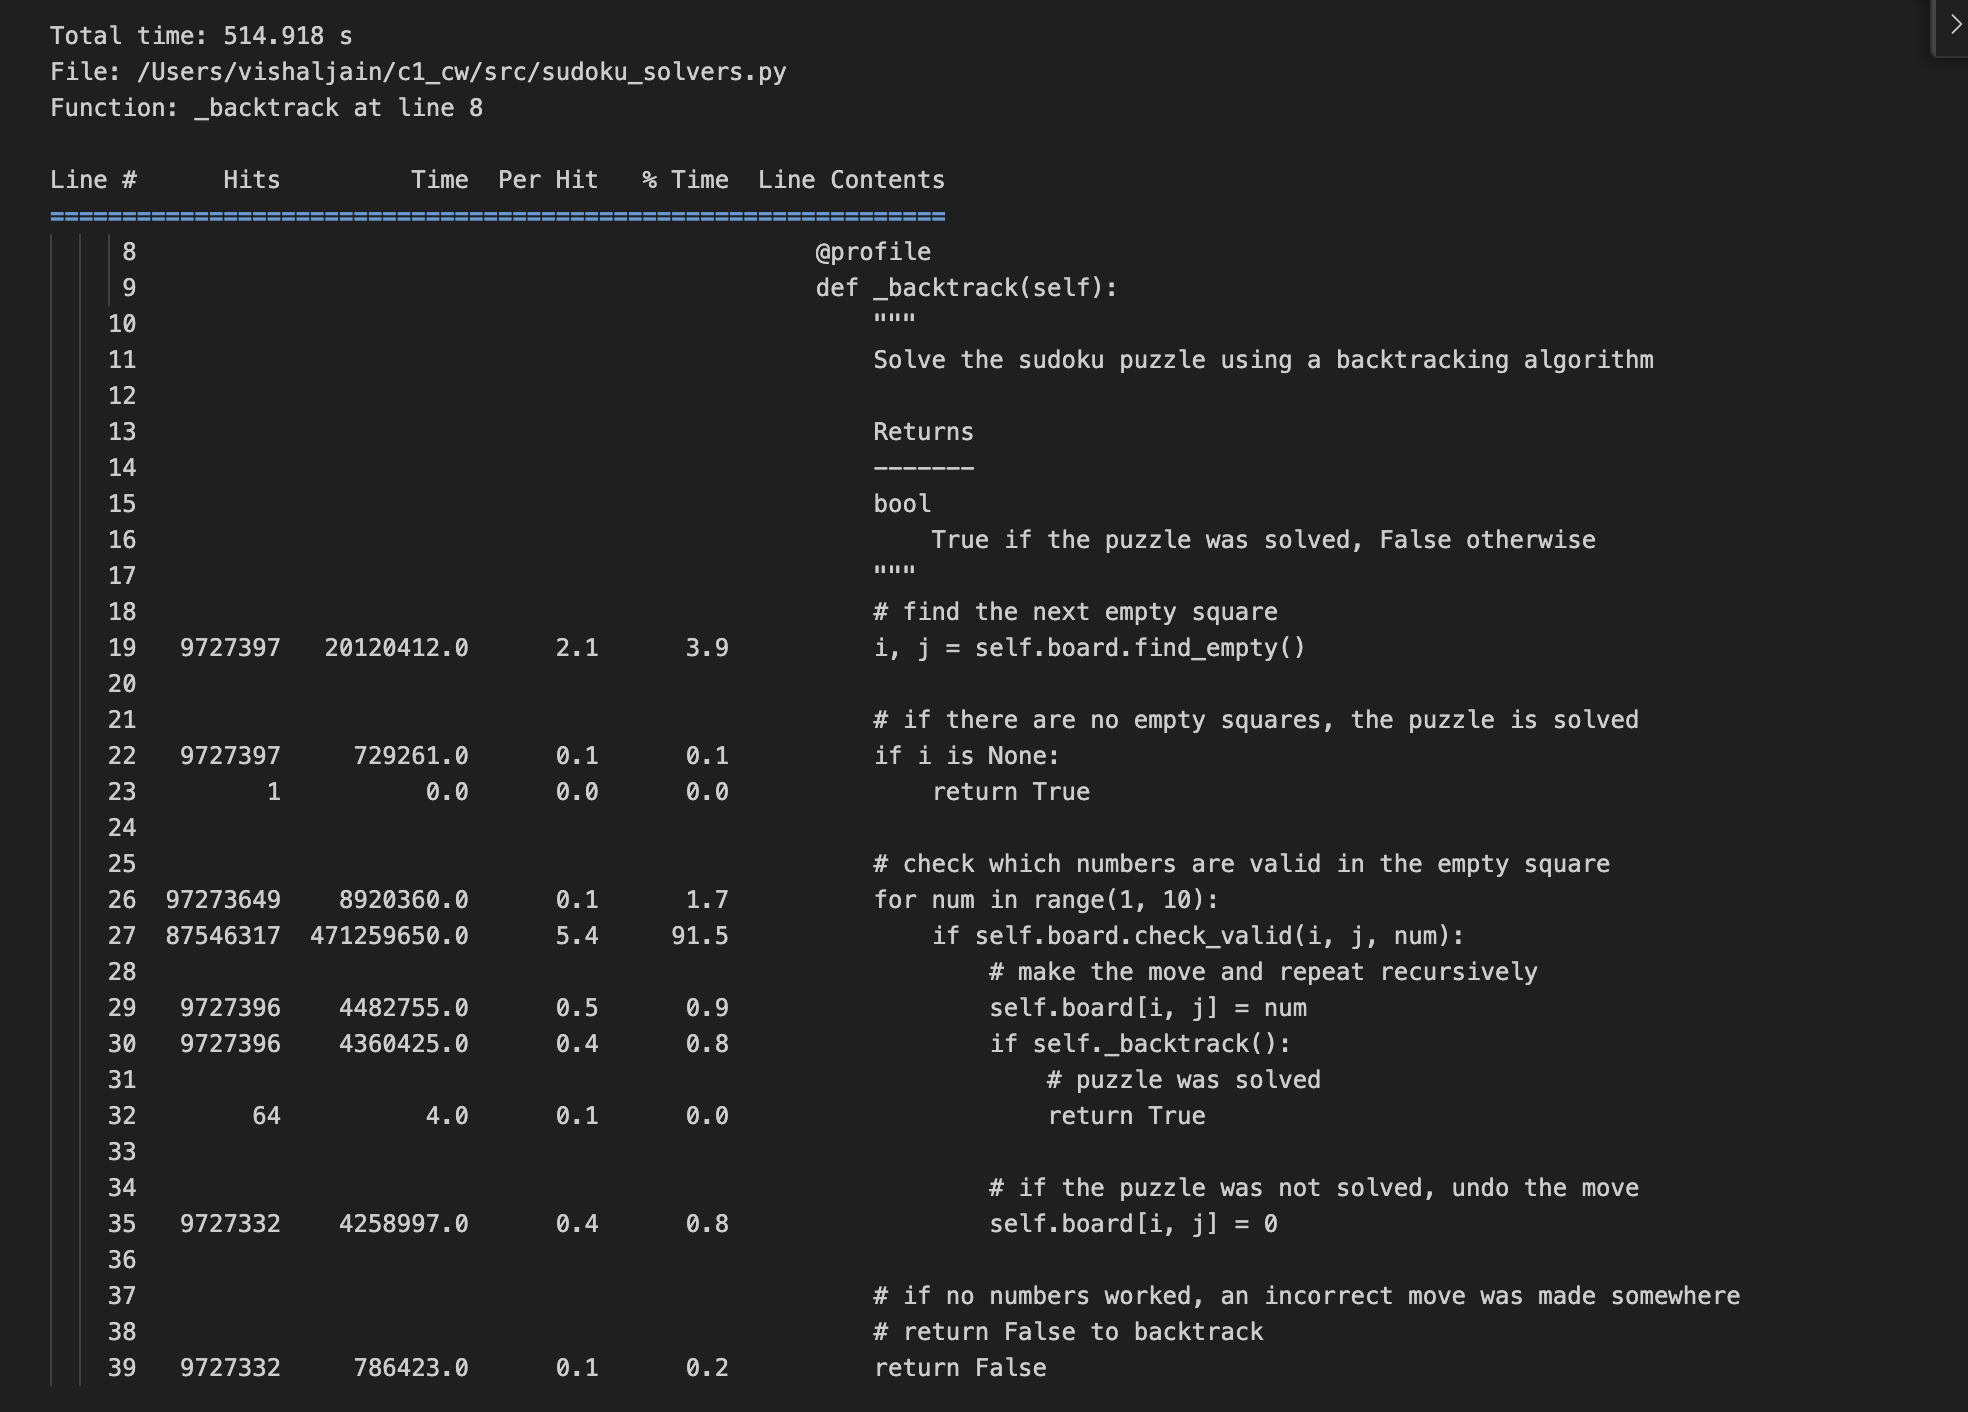
\includegraphics[width=1\textwidth]{figs/bt_line_profile_before.png}
    \caption{Initial results of line profiling the backtracking method.}
    \label{fig:line_profiling_bt_initial}
\end{figure}


\begin{figure}[H]
    \centering
    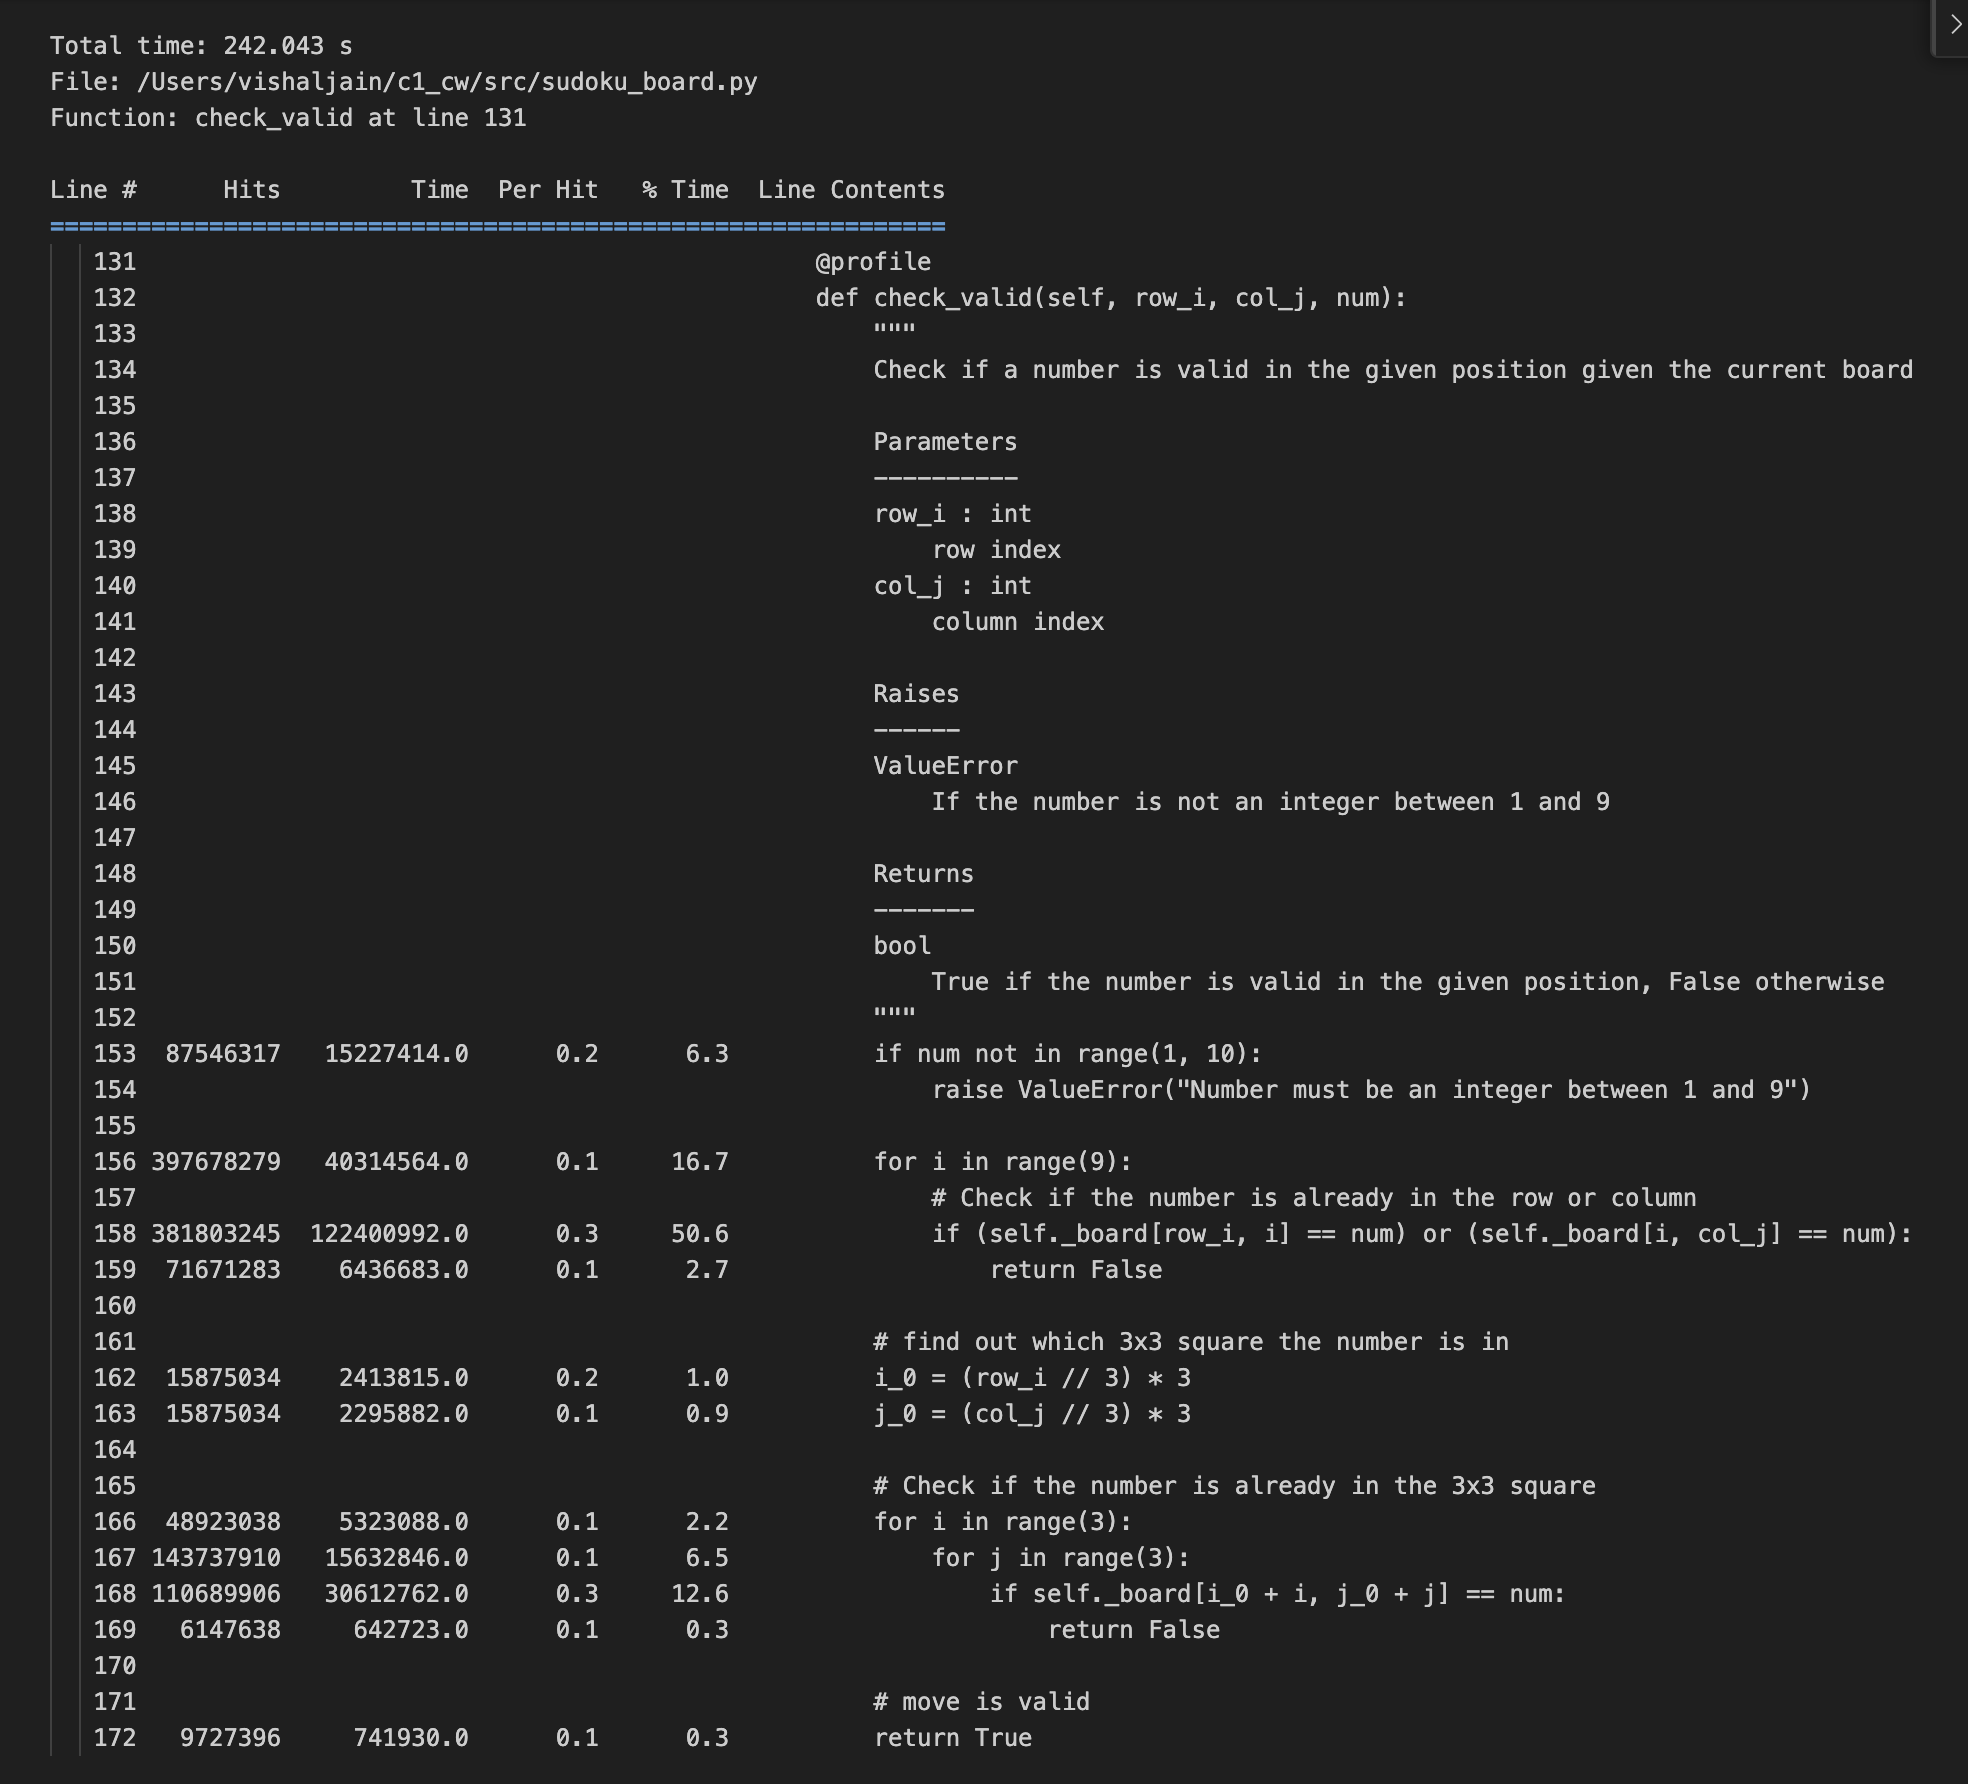
\includegraphics[width=1\textwidth]{figs/check_valid_before.png}
    \caption{Initial results of line profiling the backtracking method.}
    \label{fig:line_profiling_check_valid_initial}
\end{figure}


After modifying the \texttt{check\_valid} method to use sets instead of lists, a noticeable improvement in performance was observed. The revised function now efficiently checks if a number is valid in a given cell using sets to keep track of the numbers in each row, column and subgrid of the board. 

\begin{figure}
    \centering
    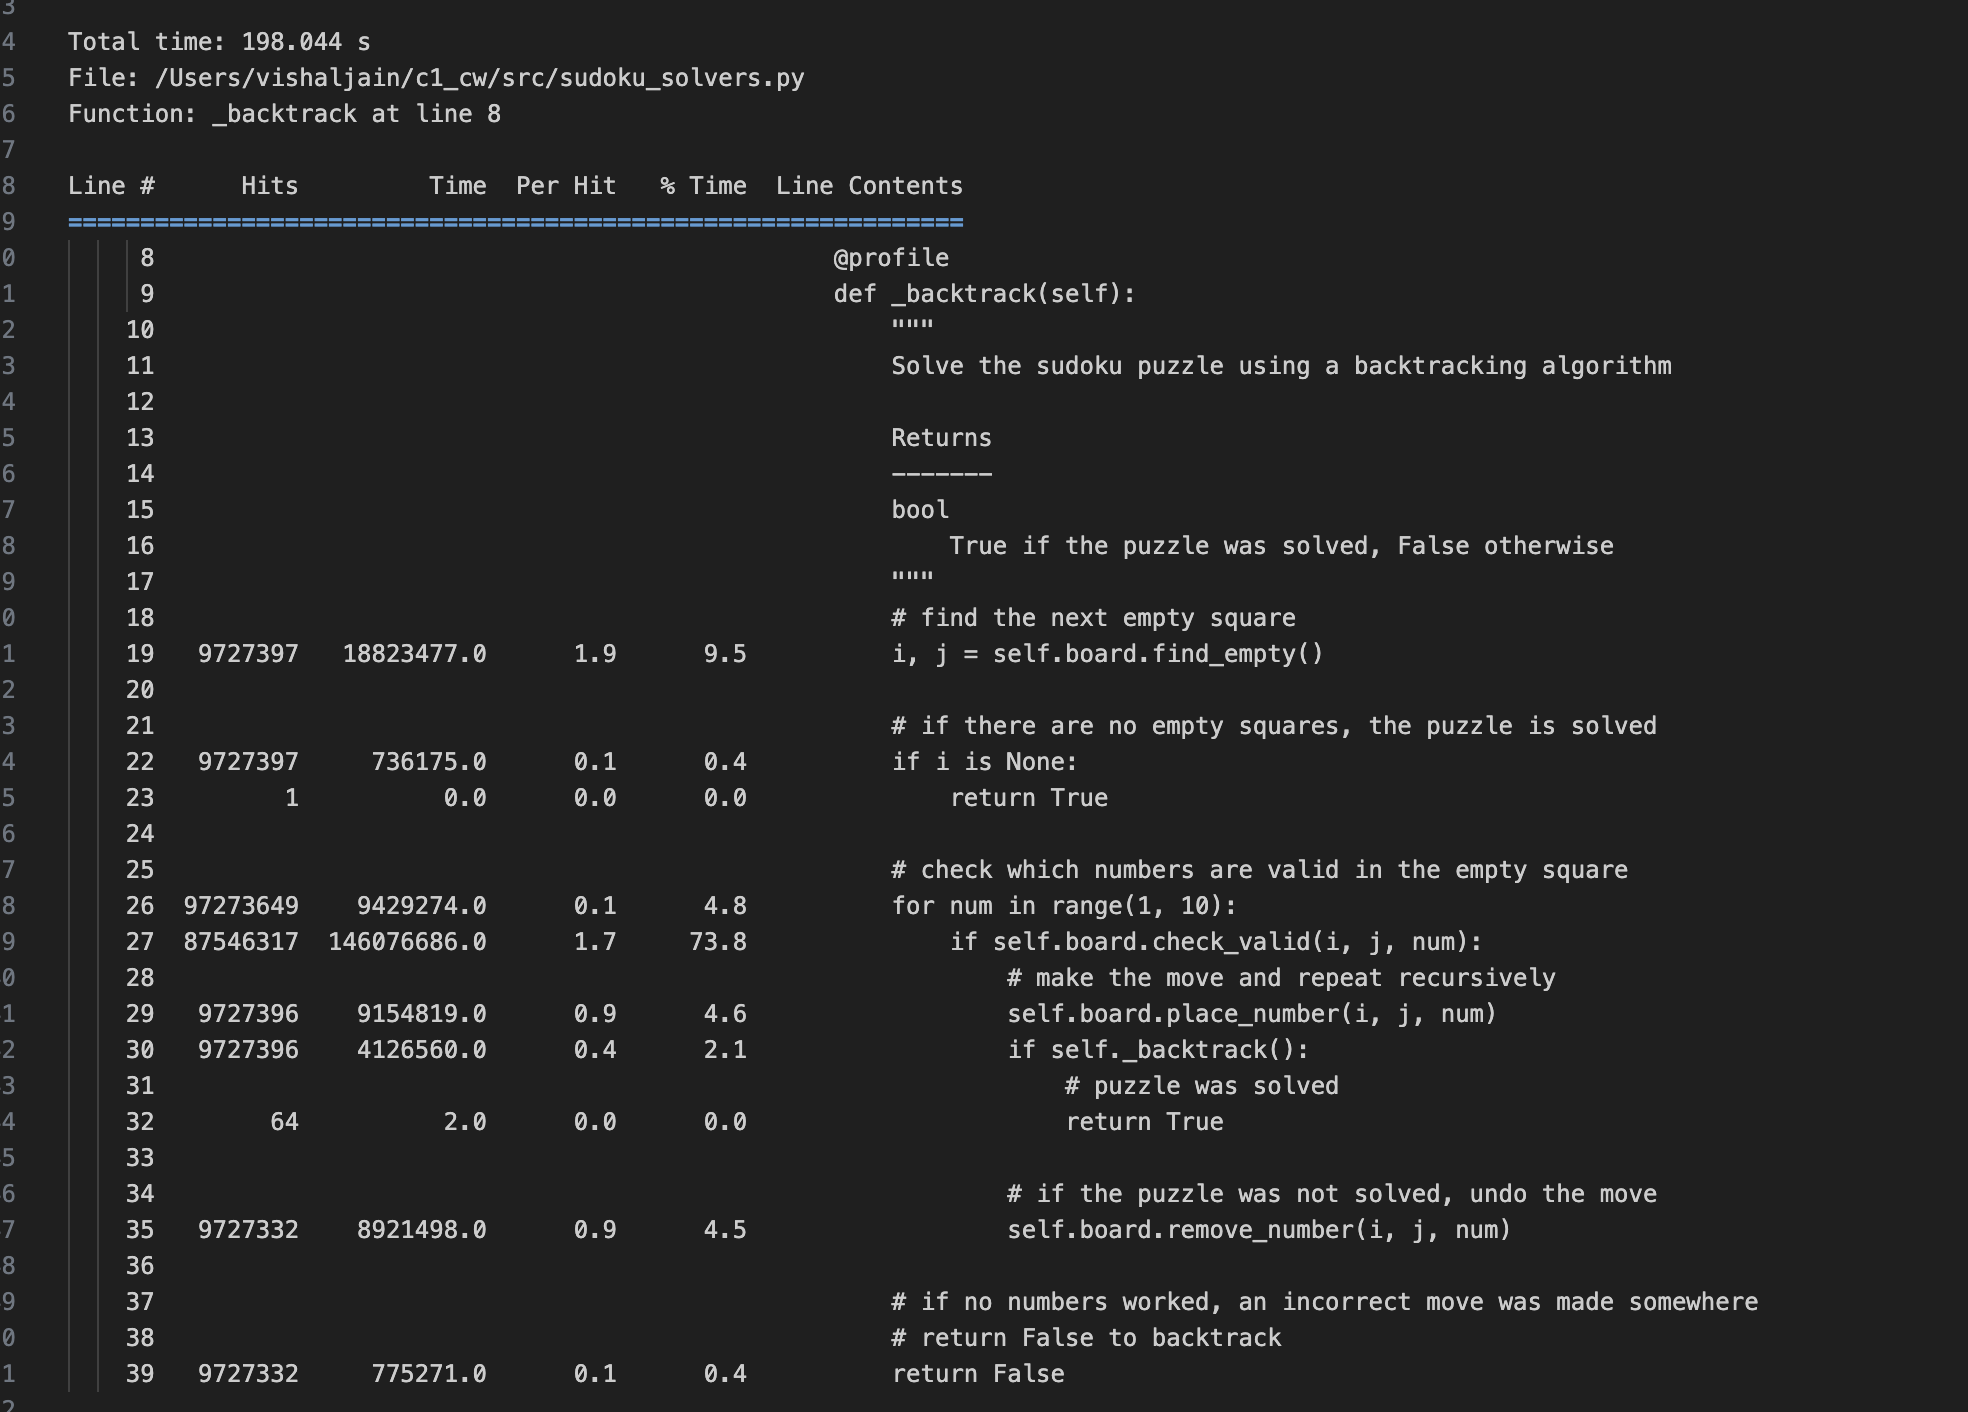
\includegraphics[width=1\textwidth]{figs/bt_line_profile_after.png}
    \caption{Results of line profiling the backtracking method after optimising the check\_valid method.}
    \label{fig:line_profiling_bt_after}
\end{figure}

\begin{figure}
    \centering
    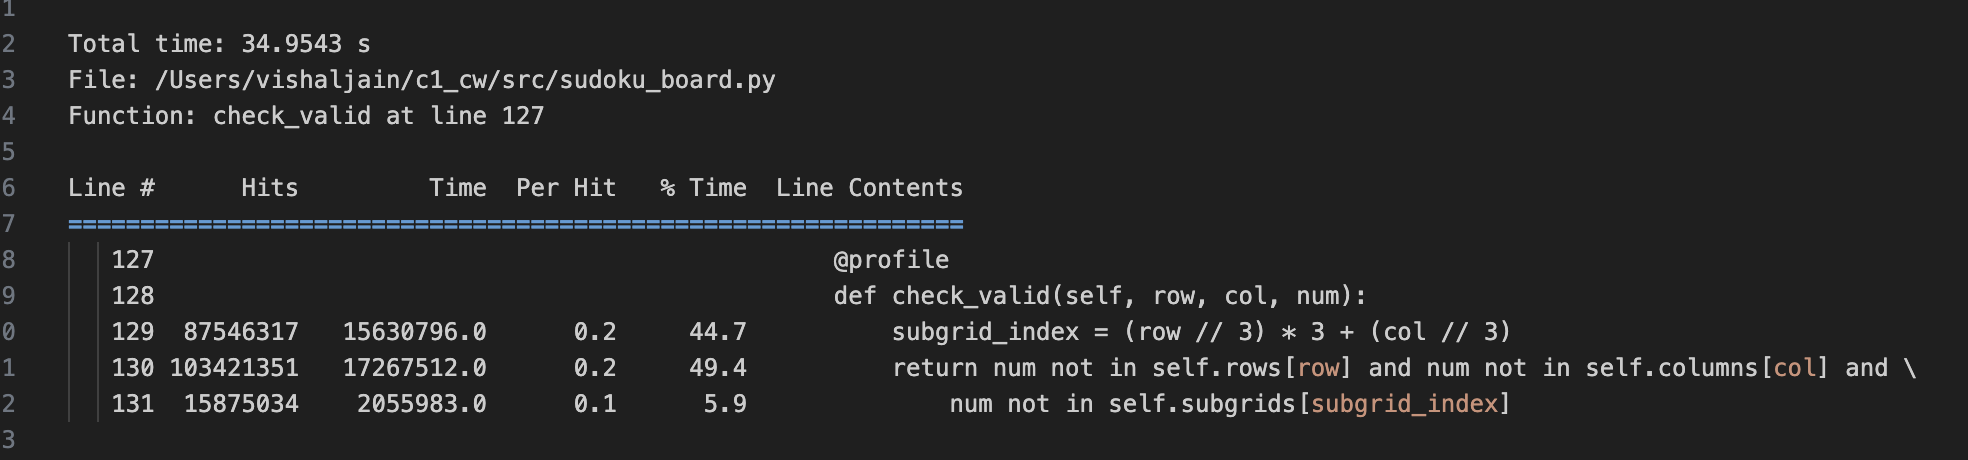
\includegraphics[width=1\textwidth]{figs/check_valid_after.png}
    \caption{Results of line profiling the check valid method after optimising the method to use sets.}
    \label{fig:line_profiling_check_valid_after}
\end{figure}


The updated \texttt{check\_valid} function, showed a reduced total execution time of 34.9543 seconds. Additionally, the total time for the texttt{\_backtrack} function dropped to 198.044 seconds. While still significant, this represents an improvement over the previous implementation. Notably, now the proportion of \texttt{\_backtrack}'s time  spent on \texttt{check\_valid} dropped to 73.8\%, indicating a more balanced distribution of computational effort compared to the initial profiling.



\section {SWE}

Error handling
Unit Tests and CI set up
Packaging and Usability

\section {Summary}
\bibliographystyle{plain}
\bibliography{mybibfile}

\end{document}
